\documentclass[12pt, a4paper]{report}
\usepackage{fullpage}
\usepackage{graphicx}
\usepackage{standalone}
\usepackage{listings}
\usepackage{float}
\usepackage{url}
\usepackage[toc,page]{appendix}
\usepackage[english]{babel}
\usepackage{color}
\usepackage{tikz}
\usepackage{framed}

\usetikzlibrary{shapes,arrows}

\begin{document}

\begin{center}

\includegraphics[scale=0.6]{images/logo-uva.png}
\vspace{30pt}


\includegraphics[scale=0.2]{images/logo-sne_black-inv-flat}
\vspace{10pt}

\Large MSc. System and Network Engineering
\vspace{100pt}

\textbf{\huge SSN Project}
\vspace{10pt}

%Welke?

\textit{\Large "SSL session key extraction from the process memory of a running Android application."}
\vspace{80pt}

\large Stamatios Maritsas - Stamatios.Maritsas@os3.nl

\large Yadvir Singh - Yadvir.Singh@os3.nl

\large Kenneth van Rijsbergen - Kenneth.vanRijsbergen@os3.nl
\vspace{80pt}

\normalsize December, 2015
\end{center}

\abstract{TLS/SSL is a widely used cryptographic protocol. The web implementation of this protocol is called HTTPS which stands for HTTP over SSL. 

Asymmetric cryptography is used by TLS/SSL to establish a secure session. When this secure session has been established it generates short term symmetric keys for each data connection in this session.

This paper will cover how dynamic code instrumentation was used to extract these symmetric keys from a running Android application and how these keys where subsequently used to decrypt captured traffic.}

\tableofcontents


\chapter{Introduction}

\section{TLS/SSL}

Transport Layer Security (TLS) and Secure Sockets Layer (SSL) are widely used protocols for securing the communication over the Internet. 

The SSL and TLS acronym are often used interchangeable to refer to transport layer encryption. Although SSL is the predecessor of TLS since 1999 and the current protocol in use is TLS, you can see in this paper that many tools and library's still use the SSL acronym. In this paper a combination of TLS and SSL will be used.
\newline
\newline
TLS is often implemented in applications such as email, browsing, VoIP and secure transactions in general. Typically when a browser connects to a secured web-page TLS is used to secure the connection. 

\noindent The way TLS sets up a secure connection is as follows: 

\begin{enumerate}
\item First by negotiating the cipher suite with the server and  authenticating the server by validating the certificate of the server with the Certificate Authority. 
\item Exchange the pre-master secret with the server using RSA key exchange. This is to establish a TLS session. 
The client will encrypt the pre-master secret with the server's public key and send it to the server. The server will then use its private key to decrypt the pre-master key.
\item Public key operations are expensive and are therefore only executed for establishing the session and authentication. For the actual transport of the data, TLS symmetric encryption is used. Both sides will generate a session-ID and a Master-key using the pre-master key. These keys will be used to encrypt the application data that will be sent over the network.
\item When a connection has been closed the session-ID and the Master-key will be destroyed.  
\end{enumerate}

\noindent So the TLS session is established using asymmetric encryption and the transportation of the traffic is secured using symmetric encryption. This means that if the session and master key where to be extracted from the local memory, then the traffic that was encrypted by this symmetric encryption can be decrypted. 

The protocol analyzer Wireshark is capable of doing just that. When provided with the right master-key and session-id it can decrypt TLS traffic.\cite{ref1,book1}

\section{Goal of this paper}

The research goal was to investigate whether it was possible to extract the TLS session key from a running Android process and to see whether those keys could be used to decrypt captured traffic. 
\newline
\noindent The corresponding research question is as follows:

\begin{framed}
\noindent \textit{How can we obtain the TLS/SSL sessions keys from the process memory of a running Android application?}
\end{framed}

\noindent The research primarily focused on the native OpenSSL library than is used by many Android applications among which the the stock browser.

\chapter{Related Work}
The article by Gursev Singh Kalra, titled ”Extracting RSAPrivate-
CrtKey and Certificates from an Android Process”, describes how to
dump X.509 certificates and construct a RSA private key (RSAPrivate-
CrtKey) from the Android application memory using Eclipse Memory
Analyzer Tool (MAT) and inspecting the Java code. This paper gave us the indication that there also might be possibilities to extract the keys from a running
process.\cite{ref1}
\newline
\newline
Also, the paper by Sally Vandeven from the SANS Institute Titled SSL/TLS: What's Under the Hood, describes how a TLS session is established, how pre-master secrets/master secrets of desktop browsers can be captured and how those captured keys can be used to decrypt captured traffic. We used the step-by-step instruction on how to use Wireshark to decrypt captured traffic using the master-key.\cite{ref2}

\chapter{Approach}
\section{Dynamic code instrumentation}

A dynamic code instrumentation tool is used to monitor, debug and log extensive information about the execution of an application. It is often used in software engineering for debugging purposes. A dynamic code instrumentation tool will "hook" into a process and "trace" certain function calls and can output or alter certain variables of the process memory while the application is running.
\newline
\newline
The rest of this paper will focus on the use of dynamic code instrumentation that is used to trace function calls to the OpenSSL library. 

\subsection{Frida}

The instrumentation tool used for this research is called Frida. Frida is an open source instrumentation tool that injects JavaScript (using Google's V8 engine) into the process space of an application. Frida can be executed from the command line but can also be controlled by using bindings (QML, Python, .NET, Node.js). These bindings makes Frida scriptable\cite{frida}. 

To use Frida on Android, a \texttt{frida-server} has to be running on the phone. This is simply done by pushing the executable to the phone and execute it through the Android Debugger shell as a process. Once the frida-server is running, it will accept commands and attach to a running Android processes that is specified in one of the commands.
\newline
\newline
The CLI (command line interface) of Frida can be used to trace specif function or you can specify some wildcards. find functions that would return the value's that we wanted. Once the command is executed by the \texttt{frida-server}, Frida will create a JavaScript file that contains two functions: \texttt{onEnter} and \texttt{onLeave} that a respectivly called when the traced function is called and when it is finished. Frida also passes the argument that are used by the traced function. Inside the \texttt{onEnter} and \texttt{onLeave} functions, the user is able to perform operations on the arguments such as printing them to the console or modification of the arguments. 
 The script contains the JavaScript code that Frida executes in the process that it hooks. The JavaScript that has been written for this research can be found at Appendix A1 and the corresponding Python binding in Appendix A2 .
\clearpage

\section{Exploring OpenSSL}
The stock Android browser uses OpenSSL. This library is open sourced and can be found on GitHub\cite{git}. The power of Frida allows us to search for functions that are called with either the master-key or session-ID as its parameter(s) or functions that return these values. The search functionality of Github allows to search on keywords such as \texttt{master-key} and \texttt{master\_key}. The keyword \texttt{master\_key} turned out to be used by functions as one of their input arguments including the following functions:

\begin{lstlisting}[frame=single, breaklines=true]
EVP_DigestUpdate(s1, s->session->master_key,s->session->master_key_length);
\end{lstlisting}

\begin{lstlisting}[frame=single, breaklines=true]
OPENSSL_cleanse(ss->master_key, sizeof ss->master_key);
\end{lstlisting}

\noindent The \texttt{EVP\_DigestUpdate} functions accepts the master-key as its second argument and the length of the key as its last argument. The \texttt{OPENSSL\_cleanse} can be found across the library and is called multiple times to clean data. In the call depicted above, it accepts (a pointer to) the data to the master-key and a size parameter. 

When using Frida, the \texttt{EVP\_DigestUpdate} function is not traceable. However the \texttt{OPENSSL\_cleanse} is traceable. Due to the frequent calls to this function, we were not able to just trace this function without some filtering. The size parameter can help hereby as the master-key length is fixed at 48 bytes. This allows us to filter function calls to the \texttt{OPENSSL\_cleanse} function where the second parameter equals 48. Test however show that there is still a lot of garbage after filtering. This is due to cleaning of data chunks that also have the same size or the removal of old sessions from which the master-key is has to be cleaned. 


\noindent Next we looked where \texttt{OPENSSL\_cleanse} function with the master-key as parameter is called. It turned out to be inside the following function:

\begin{lstlisting}[frame=single, breaklines=true]
void SSL_SESSION_free(SSL_SESSION *ss)
\end{lstlisting}

This function is responsible for removing the session from the memory. It accepts a pointer to session that needs to be cleared. Besides the \texttt{OPENSSL\_cleanse} function, another interesting function is called within \texttt{SSL\_SESSION\_free}:

\begin{lstlisting}[frame=single, breaklines=true]
OPENSSL_cleanse(ss->session_id, sizeof ss->session_id);
\end{lstlisting}

This functions removes the session-ID and the same filtering trick as with the master-key size can be applied (filtering on 32 bytes instead of 48). This Method, as described earlier, also suffers from polluted results.
\newline
\newline
\noindent Another way to extract the master-key and session-ID is to look at the session object (\texttt{*ss}) which is passed as an argument to the \texttt{SSL\_SESSION\_free} function. This session object contains all the information about the session among which the master-key and session-ID. Using Frida it is possible to retrieve the memory location of the session object by extracting tracing the \texttt{SSL\_SESSION\_free} function. The same holds for the function calls to \texttt{OPENSSL\_cleanse} where the memory address of \texttt{ss->session\_id} and \texttt{ss->master\_key} can be retrieved. When comparing the memory locations, the following offsets can be found:

\tikzstyle{arrow} = [thick,->,>=stealth]
\tikzstyle{session} = [rectangle, rounded corners, minimum width=4cm, minimum height=1cm,text centered, draw=black, fill=green!30]
\tikzstyle{key} = [rectangle, rounded corners, minimum width=3cm, minimum height=1cm,text centered, draw=black, fill=orange!30]
\tikzstyle{hi} = [rectangle, rounded corners, minimum width=3cm, minimum height=1cm,text centered, draw=black, fill=blue!25]

\begin{figure}[!h]
\centering
\begin{tikzpicture}[node distance=3cm]

\node (sessionObject) [session] {SSL\_SESSION};
\node (masterKey) [key,below of=sessionObject,xshift=-0.5cm, left] {master\_key};
\node (sessionID) [hi,below of=sessionObject,xshift=0.5cm, right] {session\_id};


\draw [arrow] (sessionObject) -- node[anchor=east] {+20} (masterKey);
\draw [arrow] (sessionObject) -- node[anchor=west] {+72} (sessionID);
\end{tikzpicture}
\caption{Master-key and session-ID offset.}
\end{figure}
\noindent With these offsets it is possible to extract the master-key and session-ID from the session object. This now allows us to trace functions that accept the session object rather than the master-key or session-ID, which broadens the number of functions that are of interest. 
\newline
\newline
One of the function that is called on the initialization of a HTTPS connection is:
\begin{lstlisting}[frame=single, breaklines=true]
SSL_CTX_add_session(SSL_CTX *s, SSL_SESSION *c)
\end{lstlisting}
The second argument that is accepted by the \texttt{SSL\_CTX\_add\_session} function is the session object (\texttt{*c}). To extract the master key from this function, the memory location of the session object needs to be incremented by 20. The newly computed address now points to the memory location of the master-key from which the first 48 bytes need to be read. This raw data needs to undergo some processing before the master-key can be seen, see appendix A1 for the script used. The same procedure can be repeated to extract the session-ID. The only difference is the offset. 
This function turned out to be the best hook point to retrieve the master-key and session-ID as it is called on the initialization of a session rather, opposite to the \texttt{OPENSSL\_cleanse} and \texttt{SSL\_SESSION\_free} functions that are called when the session is discarded.

\chapter{Experiments}
\section{Setup}

After deciding that dynamic code instrumentation was going to be used (particularly Frida), we had to set up an experimental environment. Briefly speaking, the main components of this environment were a desktop workstation and an Android smart phone.  

The paragraphs below will go into more detail on how the the experimental environment was set up.


\subsection{OpenSSL HTTPS debug server}

First of all, we had to set up a simple \texttt{OpenSSL HTTPS server}. This server helped us verifying the master-key and session-ID. The debug server would output the master-key and session-ID in the browser and by tracing several OpenSSL library functions we could search for and verify if we extracted the correct values.

In essence, we have been through the following procedure:

\begin{enumerate}
\item Create two certificates, which will be used by the \texttt{OpenSSL s\_server}:
\begin{lstlisting}[frame=single, breaklines=true]
openssl req -x509 -newkey rsa:2048 -keyout key.pem -out
cert.pem -days 365 -nodes	
\end{lstlisting}	

\item Starting the \texttt{OpenSSL s\_server}:
\begin{lstlisting}[frame=single, breaklines=true]
openssl s_server -key key.pem -cert cert.pem -accept 44330
-www -no_ticket
\end{lstlisting}

\item Accessing the \texttt{s\_server} via the built-in Android smart phone's browser:
\begin{lstlisting}[frame=single, breaklines=true]
https://145.100.102.106:44330
\end{lstlisting}
The IP \texttt{145.100.102.106} represents the desktop workstation and \texttt{Port:44330} is the default port that we want our debug server to operate on.  

\end{enumerate}

\subsection{Traffic capture}

In this subsection the two applications that where used to analyse the TLS/SSL network packets are explained. First of all we needed to capture the TLS/SSL traffic that was being generated while browsing. To do this we set up a proxy server. On the same machine the proxy server was running we set up Wireshark. This would capture and monitor the traffic that was incoming on the proxy's server port.


\subsubsection{Proxy server}

For the proxy server we used Tinyproxy, which is a light-weight HTTP/HTTPS proxy daemon that doesn't require anything more than a POSIX environment (Unix-like system) to operate on. It was designed to be a fast and small proxy and for our experiment this proxy was sufficient.

\begin{enumerate}
\item Installation \\
Installing Tinyproxy using the Advanced Packaging Tool:
\begin{lstlisting}[frame=single, breaklines=true]
sudo apt-get install tinyproxy			
\end{lstlisting}	

\item Configuration \\
Inside its configuration file, which is located at \texttt{/etc/tinyproxy.conf} we needed to add the entry:
\begin{lstlisting}[frame=single, breaklines=true]
Allow 145.100.102.66/27			
\end{lstlisting}		
which was the IP that the Android smart phone was getting, while it 			was being connected to our SNE Lab WiFi (always the same). The \texttt{Allow} tag helps the user easily customize the authorization controls. 

\item Start/Stop service \\
Restarting Tinyproxy server right after every change inside its configuration file using the following pair of commands:
\begin{lstlisting}[frame=single, breaklines=true]
sudo /etc/init.d/tinyproxy stop
sudo /etc/init.d/tinyproxy start			
\end{lstlisting}

\item Debugging \\
In order to be able to check smart phone's connection on the proxy server we were viewing Tinyproxy's log file using the following command (as a superuser):
\begin{lstlisting}[frame=single, breaklines=true]
tail -f /var/log/tinyproxy/tinyproxy.log
\end{lstlisting}
\end{enumerate}

Finally, using the following command we simply confirmed that eventually Tinyproxy was up and running at \texttt{Port:8888}, which is its default:

\begin{lstlisting}[frame=single, breaklines=true]
netstat -ntulpn | grep :8888
tcp    0   0 0.0.0.0:8888    0.0.0.0:*    LISTEN  3638/tinyproxy
\end{lstlisting}

\subsubsection{Wireshark}

As we mention above, using Wireshark we were able to monitor all the traffic  that is destined for the proxy server on Port 8888. As we were interested only in the TLS/SSL traffic, we created a filter on Wireshark to make testing and filtering more easy. The filter's string was set to \texttt{tcp.port==8888 \&\& ssl}. Another change made to Wireshark is the default port for the SSL/TLS traffic which is set to 443. As the debug server runs on port 44330, we manually added this port to the default port for SSL/TLS traffic.  

Another capability of Wireshark that we used was the ability to decrypt an SSL session, using simple text file with the correct combination of \texttt{RSA Session-ID} and the \texttt{Master-Key}. The format that is accepted by Wireshark is as follows:
\begin{lstlisting}[frame=single, breaklines=true]
RSA Session-ID:<value> Master-Key:<value>		
\end{lstlisting}

\subsection{Desktop/Smart phone Setup}

Let us now describe which service is running on which device. Firstly, we should say that the already mentioned tools, such as OpenSSL HTTPS debug server, Tinyproxy server and Wireshark they are all installed on desktop workstation from which we deploy the tests and make the capturing.

In addition, another service, which is of viral importance for the scope of this project is the \textbf{Frida} server. That service has to be installed in \textbf{both} desktop workstation \textbf{and} our experimental smart phone.

\begin{table}[h]
\centering
    \begin{tabular}{ | l | l | p{5cm} |}
    \hline
    \textbf{Deployed service} & \textbf{Hosting device} \\ \hline
    OpenSSL HTTPS debug server & Desktop \\ \hline 
    Tinyproxy server & Desktop \\ \hline
    Wireshark & Desktop \\ \hline
    Frida-Server & Desktop \& Smart-phone \\ \hline
    \end{tabular}
    \caption{An association between deployed services and hosting devices.}
\end{table}

\begin{enumerate}
\item Installation on desktop workstation \\
In order to be able to use Frida's functions tracing features we had to install it first via PyPI (Python Package Index). At the terminal prompt, we simply run the following command to install Frida:
\begin{lstlisting}[frame=single, breaklines=true]
sudo easy_install frida
\end{lstlisting}
In this way, all of Frida’s PyPI dependencies are automatically installed.

\item Installation on Android smart phone \\
Firstly, we needed to have installed on our desktop machine the \texttt{adb android tool}. Android Debug Bridge (ADB) is a tool that allows a user to send a wide array of terminal commands —including but not limited to basic Linux shell commands, plus some specialty developer commands— to a phone at just about any time (as long as the user have debugging enabled on the phone). ADB is often used in conjunction with rooting or modifying a phone, like in our case.
Secondly, we had to download the latest \texttt{frida-server} for Android and get it running on our experimental smart phone:
\begin{lstlisting}[frame=single, breaklines=true]
curl -O https://build.frida.re/frida/android/arm/bin/
frida-server
adb push frida-server /data/local/tmp/
adb shell "chmod 755 /data/local/tmp/frida-server"
adb shell "/data/local/tmp/frida-server &"
\end{lstlisting}

\end{enumerate}   

\begin{figure}[h]
  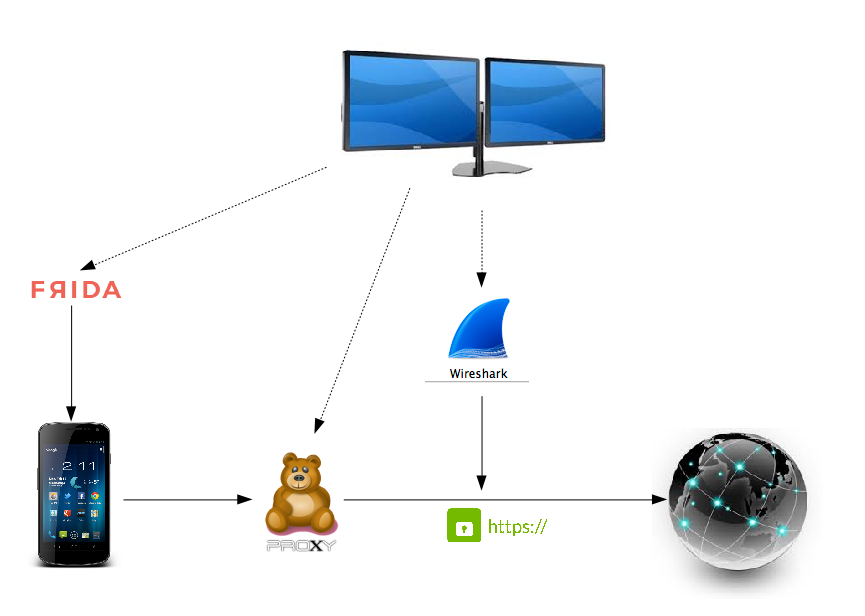
\includegraphics[width=\linewidth]{images/diagram.png}
  \caption{An overview of experimental environment.}
  %%\label{fig:boat1}
\end{figure}

\clearpage

\section{Results}



\section{Debug Server Decryption}

The first experiment was conducted on the OpenSSL debug server. The debug server shows the master-key and session-ID in the browser. This allowed us to confirm that the master-key and session-ID we extracted from the process memory were indeed the correct values.

\subsection{Result}
Using the the python script (see appendix) we were able to extract the correct master-key and session-ID. Using the found value pair we were also able to decode the captured traffic using Wireshark (see figure 4.2).


\begin{figure}[h]
\centering
  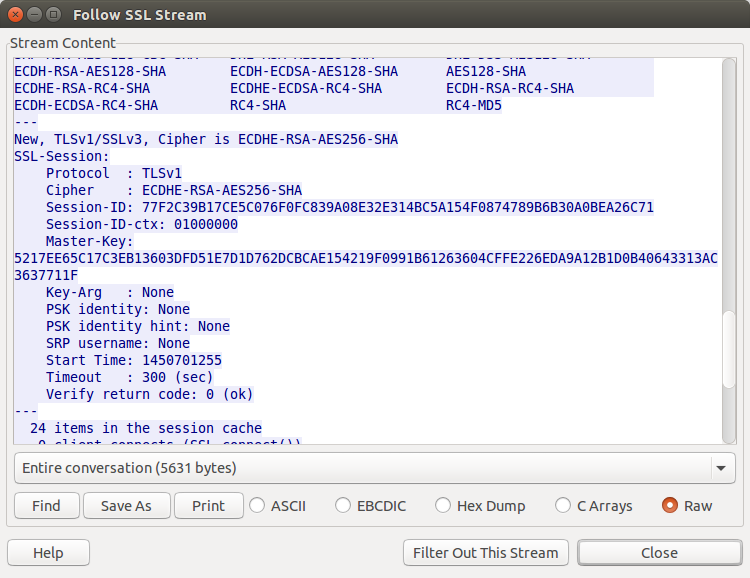
\includegraphics[scale=0.5]{images/debug.png}
  \caption{Part of the decrypted SSL stream from the debug server that shows the session-ID and master-key.}
  %%\label{fig:boat1}
\end{figure}


\clearpage
\section{Other websites}

After successfully decrypting traffic of the OpenSSL debug server, we tried the same method on different public websites (See table 4.2). 


\begin{table}[h]
\begin{tabular}{ |l|p{5cm}|p{5cm}| } 
 \hline
 Website & Cipher & Result \\ \hline 
 OpenSSL debug server & TLS\_ECDHE\_RSA\_WITH \_AES\_256\_CBC\_SHA & Full decryption \\ \hline
 
 https://bb.vu.nl & TLS\_RSA\_WITH\_RC4\_128 \_MD5 & HTTP headers + Password \\ \hline
 
 https://mijn.ing.nl & TLS\_ECDHE\_RSA \_WITH\_AES\_128\_CBC\_SHA & HTTP headers + Password \\ \hline

 https://digid.nl/inloggen & TLS\_RSA\_WITH \_AES\_128\_CBC\_SHA & Full decryption + Password \\ \hline

 https://hotmail.com & TLS\_ECDHE\_RSA \_WITH\_AES\_256\_CBC\_SHA & Full decryption + Password \\ \hline

 https://duo.nl & TLS\_RSA\_WITH\_AES \_128\_CBC\_SHA & Full decryption \\ \hline
 
 https://os3.nl & TLS\_ECDHE\_RSA\_WITH \_AES\_128\_CBC\_SHA & Not able to decrypt \\ \hline

\end{tabular}

\caption{Table of tested websites and their decryption results.}
\end{table}


The first public website that was tested was \textit{https://bb.vu.nl}. With the acquired session-ID and master-key it was possible to decrypt the HTTP headers which included the password and user-name of a log in attempt. The actual page contents were not decryptable. The same holds for the banking website \textit{ https://mijn.ing.nl}.
\newline
\newline
The third website, \textit{https://digid.nl/inloggen} was fully decryptable and the password could be recovered from the HTTP headers. We noticed that when you connect to this website, it will send multiple \textit{server hello} packets that contain the same session-ID but the master-key differs for each packet. This means that instead of decrypting the entire page with a single value pair, we had to decrypt multiple parts of the web-page and glue them together afterwards.
\newline
\newline
Both \textit{https://hotmail.com} and \textit{https://duo.nl} were decryptable using a single master-key and session-ID. In the case of \textit{https://hotmail.com}, the email address and password could be extracted from the HTTP header. 
\newline
\newline
The last website website we tested was \textit{https://os3.nl}, the web page of our master program. Although we found several pairs of session-IDs that where visible in the \textit{server hello} packets, none of the corresponding master-keys were able to decrypt the traffic.

\chapter{Conclusion}


Using dynamic code instrumentation we were able to extract SSL session keys from the process memory of the Android stock browser. Using Frida, we could trace function calls to the OpenSSL library. After some searching we found several function that accept the master-key as one of their arguments. When tracing these function, the results where polluted by incorrect master-keys. As a second approach, the master-key and session-ID could be extracted from the session object which is frequently passed to many functions in the OpenSSL library. 
\newline
\newline
The OpenSSL function \texttt{SSL\_CTX\_add\_session(SSL\_CTX *s, SSL\_SESSION *c)} proved to be the function that was both traceable and from which the address of the session object could be retrieved. Using fixed offsets, the master-key and session-ID were extractable and most of the SSL traffic could be decrypted using the found key(s).


\chapter{Attack Limitations \& Future work}


\section{Attack Limitations}
The use of Frida puts some constrains on the attack possibilities. First, the Android phone needs to be rooted. The frida-server is not able to inject itself unless running as root. Secondly, Frida's documentation is scarce and a lot of trial and error is involved. Also, Frida was not able to trace all functions of the OpenSSL library and the error returned wasn’t usable to find the specific cause.  
\newline
\newline
The second limitation is the ability to capture network traffic. In the test-setup we used a proxy server and we explicitly configured the phone to route all its traffic through that proxy server. In the real-world case, an attacker would need to somehow capture the traffic (e.g. ARP spoofing). When not on the same network as the victim the problem of capturing data becomes harder. 
\newline
\newline
The third limiting factor is the fact that the Android phone needs to be physically connected to a computer (the computer needs to run Android Debug Bridge (adb)). Although posts on the Github repository indicate that it is possible to attach to the frida-server over ssh, it is not yet been documented.   


\section{Future work}

As future work, research can be done on the wireless use of Frida. There have been forum postings about making a remote connection with Frida over SSH, but this has not been officially documented yet and is also not an official feature of Frida.
\newline
\newline
The second improvement could be the use of Frida without root access. Cedric Van Bockhaven mentioned that: "By decompiling, injecting a shared object, and then repackaging." you are able to use Frida without root access.



\bibliographystyle{plain}
\bibliography{bibliography}

\begin{appendices}

\chapter{}
\section{Frida Script - JavaScript}


\definecolor{javared}{rgb}{0.6,0,0} % for strings
\definecolor{javagreen}{rgb}{0.25,0.5,0.35} % comments
\definecolor{javapurple}{rgb}{0.5,0,0.35} % keywords
\definecolor{javadocblue}{rgb}{0.25,0.35,0.75} % javadoc
 
\lstset{language=Java,
basicstyle=\ttfamily,
keywordstyle=\color{javapurple}\bfseries,
stringstyle=\color{javared},
commentstyle=\color{javagreen},
morecomment=[s][\color{javadocblue}]{/**}{*/},
tabsize=2,
showspaces=false,
showstringspaces=false}

\begin{lstlisting}[frame=single, breaklines=true]
/*
 * Auto-generated by Frida. Please modify to match the signature of SSL_CTX_add_session.
 * This stub is currently auto-generated from manpages when available.
 *
 * For full API reference, see: http://www.frida.re/docs/javascript-api/
 */

{
    /**
     * Called synchronously when about to call SSL_CTX_add_session.
     *
     * @this {object} - Object allowing you to store state for use in onLeave.
     * @param {function} log - Call this function with a string to be presented to the user.
     * @param {array} args - Function arguments represented as an array of NativePointer objects.
     * For example use Memory.readUtf8String(args[0]) if the first argument is a pointer to a C string encoded as UTF-8.
     * It is also possible to modify arguments by assigning a NativePointer object to an element of this array.
     * @param {object} state - Object allowing you to keep state across function calls.
     * Only one JavaScript function will execute at a time, so do not worry about race-conditions.
     * However, do not use this to store function arguments across onEnter/onLeave, but instead
     * use "this" which is an object for keeping state local to an invocation.
     */
    onEnter(log, args, state) {
        log("SSL_CTX_add_session(" + "" + ")");

		a = args[1].toInt32()
		log(a)
		b = a + 20


		c = new NativePointer(b)

		key = Memory.readByteArray(c, 48);

		//The ArrayBuffer needs to be converted to decimals. 
		tempConvert = new Uint8Array(key);
		arr = [];


		//Convert decimal to hex. 
		for(i = 0; i < 48; i++){
			arr[i] = ("0" + tempConvert[i].toString(16).toUpperCase()).substr(-2);
		}


			//Print the key
		log (arr[0] +arr[1] +arr[2] +arr[3] +arr[4] +arr[5] +arr[6]  + arr[7] +arr[8] +arr[9]+arr[10] +arr[11] +arr[12]+arr[13] +arr[14] +arr[15] +arr[16] +arr[17] +arr[18]  + arr[19] +arr[20] +arr[21]+arr[22] +arr[23] +arr[24]+arr[25] +arr[26] +arr[27] +arr[28] +arr[29] +arr[30]  + arr[31] +arr[32] +arr[33]+arr[34] +arr[35] +arr[36] +arr[37] +arr[38] +arr[39] +arr[40] +arr[41] +arr[42]  + arr[43] +arr[44] +arr[45]+arr[46] +arr[47])


		log("Session ID:")

		a = args[1].toInt32()

		b = a + 72

		c = new NativePointer(b)

		key = Memory.readByteArray(c, 32);

		//The ArrayBuffer needs to be converted to decimals. 
		tempConvert = new Uint8Array(key);
		arr = [];


		//Convert decimal to hex. 
		for(i = 0; i < 32; i++){
			arr[i] = ("0" + tempConvert[i].toString(16).toUpperCase()).substr(-2);
		}


		//Print the key
		log (arr[0] +arr[1] +arr[2] +arr[3] +arr[4] +arr[5] +arr[6]  + arr[7] +arr[8] +arr[9]+arr[10] +arr[11] +arr[12]+arr[13] +arr[14] +arr[15] +arr[16] +arr[17] +arr[18]  + arr[19] +arr[20] +arr[21]+arr[22] +arr[23] +arr[24]+arr[25] +arr[26] +arr[27] +arr[28] +arr[29] +arr[30]  + arr[31])

    },

    /**
     * Called synchronously when about to return from SSL_CTX_add_session.
     *
     * See onEnter for details.
     *
     * @this {object} - Object allowing you to access state stored in onEnter.
     * @param {function} log - Call this function with a string to be presented to the user.
     * @param {NativePointer} retval - Return value represented as a NativePointer object.
     * @param {object} state - Object allowing you to keep state across function calls.
     */
    onLeave(log, retval, state) {
    }
}
\end{lstlisting}






% Define Colors
\definecolor{eclipseBlue}{RGB}{42,0.0,255}
\definecolor{eclipseGreen}{RGB}{63,127,95}
\definecolor{eclipsePurple}{RGB}{127,0,85}
 
% Set Language
\lstset{
  basicstyle=\small\ttfamily, % Global Code Style
  captionpos=b, % Position of the Caption (t for top, b for bottom)
  extendedchars=true, % Allows 256 instead of 128 ASCII characters
  tabsize=2, % number of spaces indented when discovering a tab 
  columns=fixed, % make all characters equal width
  keepspaces=true, % does not ignore spaces to fit width, convert tabs to spaces
  showstringspaces=false, % lets spaces in strings appear as real spaces
  breaklines=true, % wrap lines if they don't fit
  frame=trbl, % draw a frame at the top, right, left and bottom of the listing
  frameround=tttt, % make the frame round at all four corners
  framesep=4pt, % quarter circle size of the round corners
  commentstyle=\color{eclipseGreen}, % style of comments
  keywordstyle=\color{eclipsePurple}, % style of keywords
  stringstyle=\color{eclipseBlue}, % style of strings
}


\section{Frida script - Python}

\begin{lstlisting}[frame=single, breaklines=true]
# frida-trace -U -i SSL_CTX_add_session com.android.browser
import frida
import sys
 
# v Insert Javascript code below v
jscode = """
/**
* Use > print session.enumerate_modules(), to view all modules that are loaded in the process
*/ 
Interceptor.attach(Module.findExportByName('libssl.so', 'SSL_CTX_add_session'), {
 
onEnter: function (args) { 	
        this.fileDescriptor = args[1].toInt32();
 
	// 
	// MASTER KEY
	// 
 
	//Extract the key
	a = args[1].toInt32()
	b = a + 20
	c = new NativePointer(b)
	key = Memory.readByteArray(c, 48);
 
	//The ArrayBuffer needs to be converted to decimals. 
	tempConvert = new Uint8Array(key);
	arr = [];
	for(i = 0; i < 48; i++){
		arr[i] = ("0" + tempConvert[i].toString(16).toUpperCase()).substr(-2);
		}
 
 
	//
	// SESSION KEY
	//
 
	//Extract the key
	a = args[1].toInt32()
	b = a + 72
	c = new NativePointer(b)
	key = Memory.readByteArray(c, 32);
 
 
	//The ArrayBuffer needs to be converted to decimals. 
	tempConvert = new Uint8Array(key);
	arr2 = [];
	for(i = 0; i < 32; i++){
		arr2[i] = ("0" + tempConvert[i].toString(16).toUpperCase()).substr(-2);
			}
 
 
	send ("RSA Session-ID:" +arr2[0] +arr2[1] +arr2[2] +arr2[3] +arr2[4] +arr2[5] +arr2[6]  + arr2[7] +arr2[8] +arr2[9]+arr2[10] +arr2[11] +arr2[12]+arr2[13] +arr2[14] +arr2[15] +arr2[16] +arr2[17] +arr2[18]  + arr2[19] +arr2[20] +arr2[21]+arr2[22] +arr2[23] +arr2[24]+arr2[25] +arr2[26] +arr2[27] +arr2[28] +arr2[29] +arr2[30]  + arr2[31] +" Master-Key:" +arr[0] +arr[1] +arr[2] +arr[3] +arr[4] +arr[5] +arr[6]  + arr[7] +arr[8] +arr[9]+arr[10] +arr[11] +arr[12]+arr[13] +arr[14] +arr[15] +arr[16] +arr[17] +arr[18]  + arr[19] +arr[20] +arr[21]+arr[22] +arr[23] +arr[24]+arr[25] +arr[26] +arr[27] +arr[28] +arr[29] +arr[30]  + arr[31] +arr[32] +arr[33]+arr[34] +arr[35] +arr[36] +arr[37] +arr[38] +arr[39] +arr[40] +arr[41] +arr[42]  + arr[43] +arr[44] +arr[45]+arr[46] +arr[47])
	send (" ")
},
 
onLeave(log, retval, state) {
// nothing todo here
}
 
});
"""
# ^ Insert Javascript code above ^
 
 
# console.log() vs send() in the Javascript
## you can use console.log() to output directly to the console
## use use send() which can be parsed with the on_message() method in the python script 
 
# Handles incoming messages
def on_message(message, data):
    if message['type'] == 'send':
        print(message['payload'])
    elif message['type'] == 'error':
        print(message['stack'])
 
 
 
print "\nAttached Devices:"
print "----------------------"
print frida.get_device_manager().enumerate_devices()
 
print "\nAttaching process:"
print "----------------------"
# Attach the process
# frida.get_device_manager().enumerate_devices() [device id].atach(PID/app name)
session = frida.get_device_manager().enumerate_devices() [2].attach("com.android.browser")
print frida.get_device_manager().enumerate_devices() [2].attach("com.android.browser")
 
print "\nPossible key pairs:"
print "----------------------\n"
 
# Load script
script = session.create_script(jscode)
script.on('message', on_message)
script.load()
sys.stdin.read()
 
 
 
# Sources used for this script:
#
# https://books.google.nl/books?id=UgVhBgAAQBAJ&pg=PA110&lpg=PA110&dq=frida+python+api&source=bl&ots=SWy8q9e9PU&sig=cSHShKFcICRZVuFdMwAMG0qmyHo&hl=nl&sa=X&ved=0ahUKEwjczvKdkMrJAhUEDw8KHbIkDmYQ6AEIWTAH#v=onepage&q=frida%20python%20api&f=false
# https://github.com/frida/frida-python/blob/ee890dcb4393507f4b4bfe54a8e67ef49640f9f7/src/frida/core.py
# http://blog.mdsec.co.uk/2015/04/instrumenting-android-applications-with.html


\end{lstlisting}




\end{appendices}
\end{document}